\documentclass[30pt,twocolumn,letterpaper]{article}
\usepackage{cvpr}
\usepackage{times}
\usepackage{booktabs}
\usepackage{epsfig}
\usepackage{graphicx}
\usepackage{amsmath}
\usepackage{amssymb}
\cvprfinalcopy
\def\cvprPaperID{****}
\def\httilde{\mbox{\tt\raisebox{-.5ex}{\symbol{126}}}}
\usepackage{graphicx}
\usepackage{indentfirst}
\setlength{\parindent}{2em}
\usepackage{cite}
\usepackage[colorlinks,linkcolor=red,anchorcolor=blue,citecolor=green,backref=page]{hyperref}
\author{Qilei Zhang\\\\
Jun 28 2018}
\title{Instance-aware Semantic Segmentation Via Multi-task Network Cascades}
\begin{document}
\maketitle
\begin{abstract}
  Semantic segmentation research has recently witnessed rapid progress, but many leading methods are unable to identify object instances.
\end{abstract}
\section{Introduction}
Since the development of fully convolutional networks, the accuracy of semantic segmentation has been improved rapidly thanks to deeply learned features, large-scale annotations , and advanced reasoning over graphical models. Nevertheless, FCNs and improvements are designed to predict a category label for each pixel, but are unaware of individual object instances\cite{Briggs2013Instance}. \\
\begin{figure}[htbp]
\small
\centering
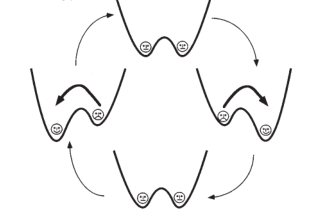
\includegraphics[width=20em]{000.png}
\caption{Illustrations of common multi-task learning (left) and our multi-task cascade (right).}
\label{fig:lable}
\end{figure}\\
\section{Related Work}
Object detection methods involve predicting object bounding boxes and categories\cite{Jankovic2015Context}.In SPPnet and Fast RCNN, the convolutional layers of CNNs are shared on the entire image for fast computation. Faster R-CNN exploits the shared convolutional features to extract region proposals used by the detector. Sharing convolutional features leads to substantially faster speed for object detection systems\cite{Miledi2016How}.\\
\begin{figure}[htbp]
\small
\centering
\includegraphics[width=20em]{001.png}
\caption{Multi-task Network Cascades for instance-aware semantic segmentation. At the top right corner is a simplified illustration.}
\label{fig:lable}
\end{figure}\\
\section{Multi-task Network Cascades}
In MNC model, the network takes an image of arbitrary size as the input, and outputs instance-aware semantic segmentation results.The cascade has three stages: propos ing box-level instances, regressing mask-level instances, and categorizing each instance.These three stages are designed to share convolutional features. Each stage involves a loss term, but a later stage��s loss relies on the output of an earlier stage, so the three loss terms are not independent\cite{Zhou2014In}.
{\small
\bibliographystyle{ieee}
\bibliography{1}
}
\end{document}
